\FloatBarrier
\begin{figure}[!h]
\begin{subfigure}[t]{1\textwidth}
	\centering
	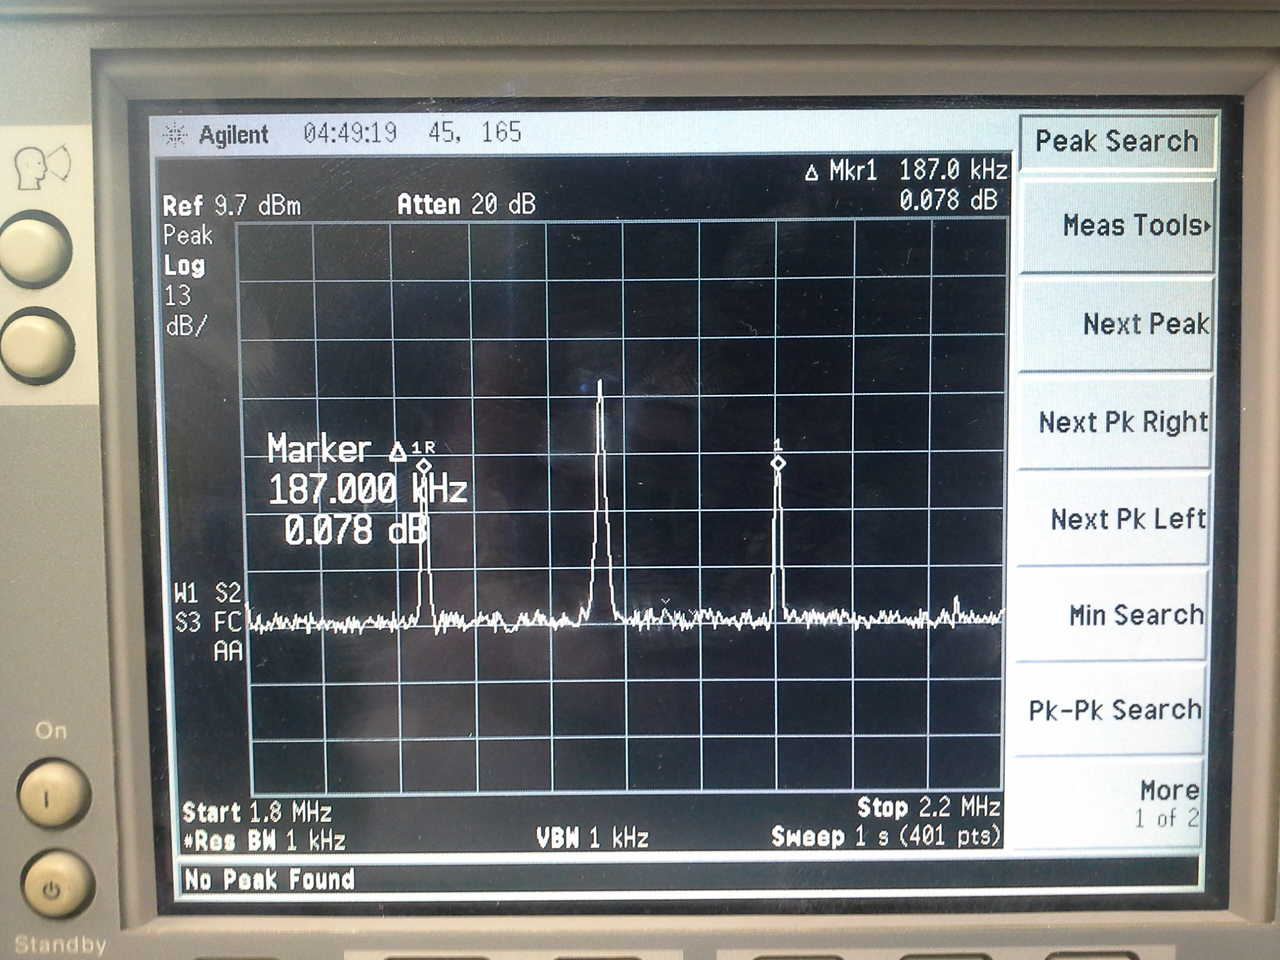
\includegraphics[scale=0.17]{../Grafiken/Frequenzspektrum_c_AmpModuliertTraeger.jpg}
	\caption{Frequenzunterschied der Seitenbänder\label{fig:frequenzspektrum_c_ampmodulierttraeger_differenz}}
\end{subfigure}
\vspace*{0.5cm}
\begin{subfigure}[t]{0.5\textwidth}
	\centering
	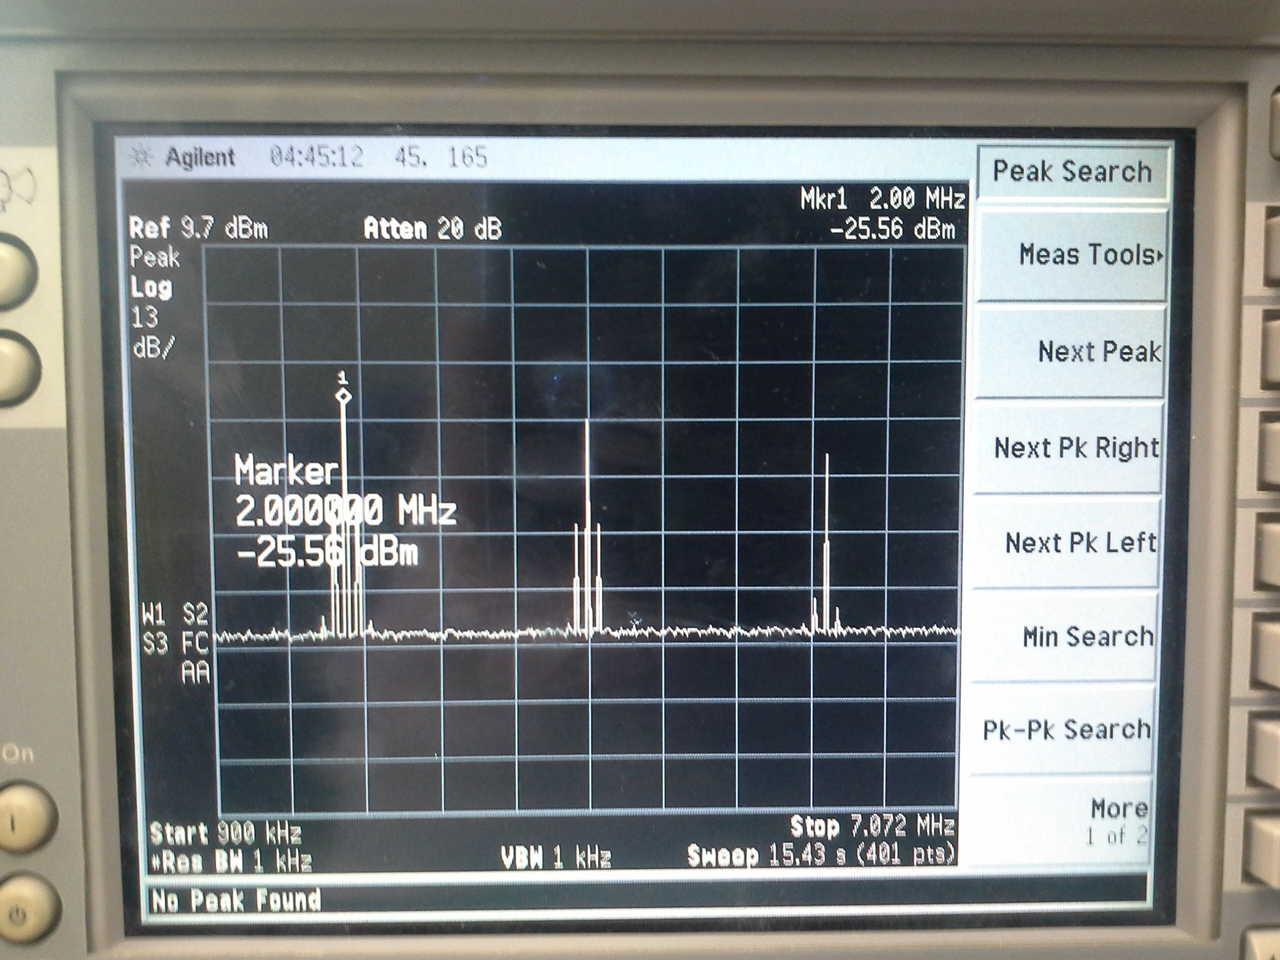
\includegraphics[scale=0.17]{../Grafiken/Frequenzspektrum_c_AmpModuliertTraeger_Oberwellen_0.jpg}
	\caption{Grundschwingung\label{fig:frequenzspektrum_c_ampmodulierttraeger_oberwellen_0}}
\end{subfigure}%
~
\begin{subfigure}[t]{0.5\textwidth}
	\centering
	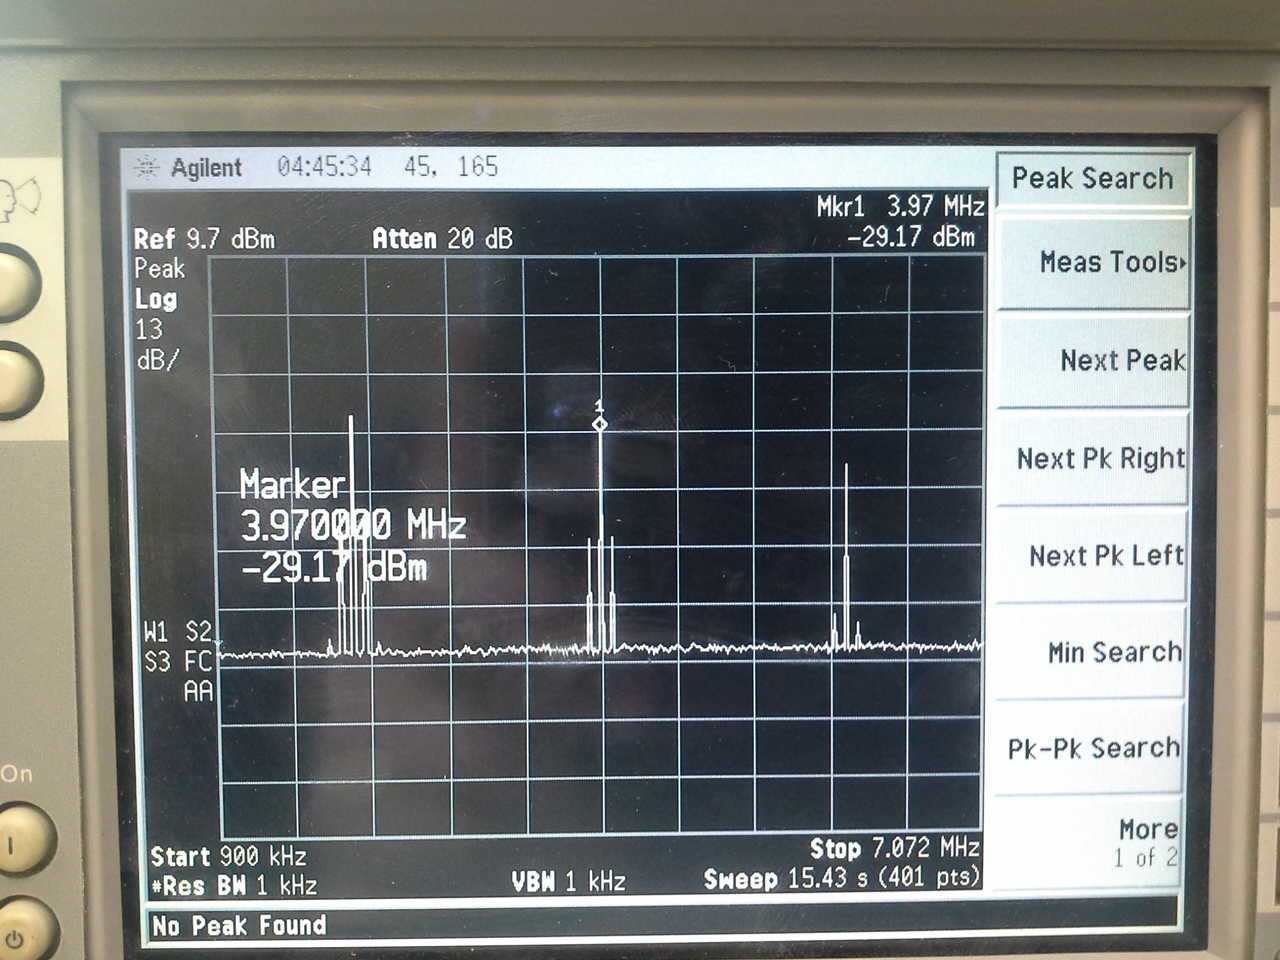
\includegraphics[scale=0.17]{../Grafiken/Frequenzspektrum_c_AmpModuliertTraeger_Oberwellen_1.jpg}
	\caption{Erste Oberschwingung\label{fig:frequenzspektrum_c_ampmodulierttraeger_oberwellen_1}}
\end{subfigure}

\caption{Frequenzspektrum der Amplitudenmodulierten Spannung mit Trägerabstrahlung. Hervorgehoben sind
	der Frequenzunterschied der Seitenbänder der Grundschwingung (a) sowie die Frequenzen der Grund- (b)
	und ersten (c) Oberschwingung.   
	\label{fig:frequenzspektrum_c_ampmodulierttraeger}}
\end{figure}
\FloatBarrier

